%	PACKAGES AND OTHER DOCUMENT CONFIGURATIONS
%----------------------------------------------------------------------------------------

\documentclass[table]{beamer}

\usetheme[numbering=fullbar]{focus}% Use the Focus theme supplied with the template
% Add option [numbering=none] to disable the footer progress bar
% Add option [numbering=fullbar] to show the footer progress bar as always full with a slide count


% peterem: font
\usefonttheme{professionalfonts} % using non standard fonts for beamer
%\usefonttheme{default} % default family is serif

% Uncomment to enable the ice-blue theme
%\definecolor{main}{RGB}{92, 138, 168}
%\definecolor{background}{RGB}{240, 247, 255}

\usepackage{array}
\usepackage{xcolor}

\usepackage{amsmath}
\usepackage{tikz}
\usetikzlibrary{matrix, fit, backgrounds}
\DeclareMathOperator{\EX}{\mathbb{E}}
\newcommand{\rr}[1]{\textcolor{red}{#1}}
\definecolor{darkgreen}{RGB}{0,135,0}
\newcommand{\gr}[1]{\textcolor{darkgreen}{#1}}

\usepackage{ulem}

%------------------------------------------------

\usepackage{booktabs} % Required for better table rules

%----------------------------------------------------------------------------------------
%	 TITLE SLIDE
%----------------------------------------------------------------------------------------

\title{Volume Estimation of \\High-Dimensional Convex Bodies}

\subtitle{MCMC Approach}

\author{Jonathan, Silvan, Manuel, Emanuel}

%\titlegraphic{\includegraphics[scale=1.25]{Images/focuslogo.pdf}} % Optional title page image, comment this line to remove it

%\institute{Institute Name \\ Institute Address}

\date{23. 05. 2020}


\newcommand{\backupbegin}{
   \newcounter{finalframe}
   \setcounter{finalframe}{\value{framenumber}}
}
\newcommand{\backupend}{
   \setcounter{framenumber}{\value{finalframe}}
}

\newcommand{\hl}[2]{
\begin{scope}[on background layer]
    \node [fit={#1}, fill=#2,inner sep=-1pt] {};
\end{scope}}


%------------------------------------------------

\begin{document}

%------------------------------------------------

\begin{frame}
	\maketitle % Automatically created using the information in the commands above
\end{frame}

%----------------------------------------------------------------------------------------
%	 SECTION 1
%----------------------------------------------------------------------------------------

%\section{Section 1} % Section title slide, unnumbered

%------------------------------------------------



\begin{frame}{Introduction}
    \onslide<1->Problem: Calculating the volume of a convex body is NP-hard.\\
    \ \\
    \onslide<2->Solution: Use randomized approximation algorithm (MCMC).
\end{frame}

\begin{frame}{Introduction}
    \onslide<1->Idea: Sample points randomly to estimate volume\\
    \ \\
    \onslide<1->\begin{center}
        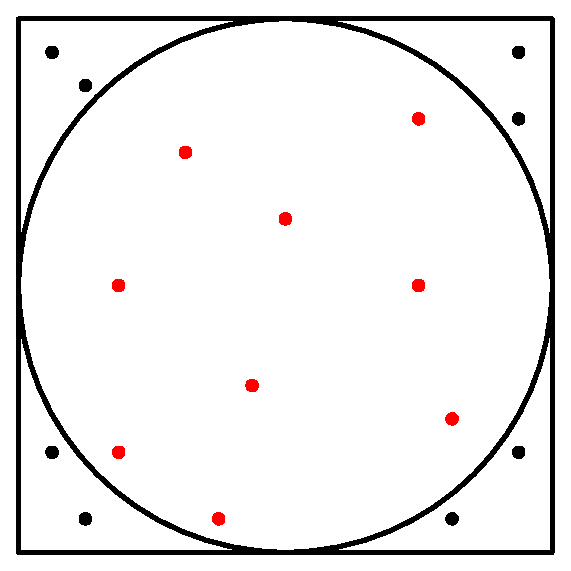
\includegraphics[width=40mm]{basic_sampling.eps}
    \end{center}
    \ \\
    \onslide<2->New problem: $\frac{Vol(\mathrm{Unit\ ball})}{Vol(\mathrm{Unit\ cube})} = O(2^{-d})$, where $d$ is the dimension
    % Label cube and ball, (samples_s / samples_c) \approx (vol_s/vol_c)
\end{frame}

\begin{frame}{Introduction}
    
    \only<1>{
        \\[0.1ex]
    }
    \only<1>{
        Consider the following convex body
    }
    \only<2>{
        \\[0.5ex]
    }
    \only<3>{
        \\[0.1ex]
    }
    
    \only<2->{
        Solution: Subdivide the body into zones to keep ratio constant
    }
    \\~\\
    
    \begin{center}
        \only<1>{
        \includegraphics[width=40mm]{basic_polytope.eps}
        }
        \only<2>{
        \includegraphics[width=45mm]{zones.eps}
        }
        \only<3>{
        \includegraphics[width=45mm]{zone_example.eps}
        }
    \end{center}
    \only<1>{
        \\~\\
        \\~\\
        \\~\\
    }
    \only<2>{
    Note: The smallest ball is fully contained and the biggest ball contains the body.
    }\only<3>{
    Each zone is the intersection of a ball with the body
    }
\end{frame}


\begin{frame}[t]{Introduction}
    \\[1.05ex]
    \onslide<1->Then sample in one zone and count how many points fall into the smaller zone
    \begin{center}
        \onslide<1->{
            \includegraphics[width=45mm]{polytope_zone_sampling_pretty.eps}
        }
    \end{center}
    \ \\
    \onslide<2->This gives us the ratio  $\frac{\mathrm{\#Total\ samples}}{\mathrm{\#Samples\ in\ {\color{red}Zone_{i}}}} \approx \frac{Vol({\mathrm{Zone_{i+1}})}}{Vol({\color{red}\mathrm{Zone_{i}}})}$
\end{frame}


\begin{frame}{Introduction}
    Doing this for all zones we can calculate the volume of the body:
\vspace{20pt}
\begin{equation*}
Vol(\mathrm{Body}) = 
\frac{Vol(\mathrm{Zone}_n)}{Vol(\mathrm{Zone}_{n-1})}
\boldsymbol{\cdot} ... \boldsymbol{\cdot}
\frac{Vol(\mathrm{Zone}_2)}{Vol(\mathrm{Zone}_1)} 
\boldsymbol{\cdot} Vol(\mathrm{Zone}_1)
\vspace{20pt}
\end{equation*}
\begin{center} 
    where $Vol(\mathrm{Zone}_1)$ is just the volume of the innermost ball.
\end{center}
\end{frame}

\begin{frame}{Introduction}
    \onslide<1->{
        How to sample uniformly at random in a zone:
        \\~\\
    }
    \begin{center}
        \only<1>{
            \hspace{2.0ex}\includegraphics[width=45mm]{sample_0.eps}%\\!\!\!\!\!\!
        }
        \only<2>{
            \hspace{1.5ex}\includegraphics[width=45mm]{direction_0.eps}%\:\!\!\!\!\!\!
        }
        \only<3>{
            \hspace{1.0ex}\includegraphics[width=45mm]{sample_1.eps}%\!\!\!
        }
        \only<4>{
            \hspace{0.5ex}\includegraphics[width=45mm]{focus_on_sample_1.eps}%\:\!\!\!
        }
        \only<5>{
            \hspace{0.5ex}\includegraphics[width=45mm]{direction_1.eps}
        }
        \only<6>{
            \includegraphics[width=45mm]{sample_2.eps}
        }
    \end{center}
\end{frame}


\begin{frame}{Compute intersections}

\begin{columns}
\column{.6\textwidth}

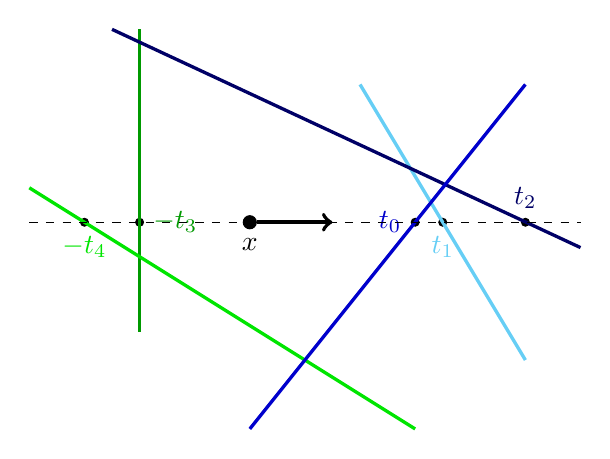
\begin{tikzpicture}[scale=.7]
\tikzstyle{node} = [draw, shape=circle, fill=black,scale=.5]
\tikzstyle{intersection} = [draw, shape=circle, fill=black, scale=.3]
  \draw 
  node (x) [label=below:{$x$}, node] at (0,0){}
  node (dir) at (1.5,0) {}
  
  node(i1) [intersection,label=left:\textcolor{black!20!blue}{$t_0$}] at (3,0) {}
  node (i2) [intersection,label=below:\textcolor{white!40!cyan}{$t_1$}] at (3.5,0) {}
  node (i3) [intersection,label=above:\textcolor{black!60!blue}{$t_2$}] at (5,0) {}
  node (i4) [intersection,label=right:\textcolor{black!40!green}{$-t_3$}] at (-2,0) {}
  node (i5) [intersection,label=below:\textcolor{black!10!green}{$-t_4$}] at (-3,0) {};
  
  \draw [black!40!green, very thick](-2,3.5) -- (-2,-2);
  \draw [black!10!green, very thick](3,-3.75) -- (-4,0.625);
  \draw [white!40!cyan, very thick](2,2.5) -- (5,-2.5);
  \draw [black!60!blue, very thick](-2.5,3.5) -- (6,-0.46);
  \draw [black!20!blue, very thick](0,-3.75) -- (5,2.5);
  \draw [dashed] (-4,0) -- (6,0);
  
  \draw [->, line width=.5mm] (x) edge (dir.center);
  %\draw [dashed] (dir) edge (end.center);
\end{tikzpicture}

\column{.4\textwidth}

\begin{equation*}
\resizebox{.9\hsize}{!}{
\left(\begin{array}{cc}
\rowcolor{black!40!green!50}
a_{0,0}  & a_{0,1} \\
\rowcolor{black!10!green!50}
a_{1,0}  & a_{1,1} \\
\rowcolor{white!40!cyan!50}
a_{2,0} & a_{2,1} \\
\rowcolor{black!60!blue!50}
a_{3,0} & a_{3,1} \\
\rowcolor{black!20!blue!50}
a_{4,0} & a_{4,1} \\
\end{array}\right) \cdot 
\left(\begin{array}{c}
x_1 + t \\
x_2
\end{array}\right) =
\left(\begin{array}{c}
\rowcolor{black!40!green!50}
b_0 \\
\rowcolor{black!10!green!50}
b_1 \\
\rowcolor{white!40!cyan!50}
b_2 \\
\rowcolor{black!60!blue!50}
b_3 \\
\rowcolor{black!20!blue!50}
b_4 \\
\end{array}\right)
 }
 \end{equation*}
\onslide<2->{

\hspace{2.9ex}solve for $t_i$ for each\\
\hspace{2.85ex}constraint $a_i$


\begin{align*}
    &\min\{\textcolor{black!20!blue}{t_0},\textcolor{white!40!cyan}{t_1},\textcolor{black!60!blue}{t_2}\} \\
    &\max\{\textcolor{black!10!green}{-t_3},\textcolor{black!40!green}{-t_4}\}
\end{align*}
}


\end{columns}
\end{frame}


\begin{frame}[t]{Compute intersections}

\begin{columns}
\column{.4\textwidth}
\begin{center}
    
    \begin{tikzpicture}[scale=.7]

	\tikzstyle{node} = [draw, shape=circle, fill=black,scale=.5]
	\tikzstyle{intersection} = [draw, shape=circle, fill=black, scale=.3]
	\tikzstyle{none} = [shape=circle, fill=none, scale=1]
	
	\only<1>{
	\draw 
	node (x1) [label=below:{$x^1$}, node] at (0,0){}
	node(t1) [label=above:{$t_i$}] at (0,2.6){}
	node(tmid) [draw=none] at (0,1.3){}
	node(tmidmid) [label=left:{$d$}, draw=none] at (0,0.6){}
	node(constr) [label=above:{\scriptsize{$a_i^\intercal x = b$}}] at (2,1.85) {}
	}
	\only<2->{
	\draw 
	node (x1) [label=below:{$x^1$}, node] at (0,0){}
	node (x2) [label=below:{$x^2$}, node] at (2,0){}
	node(t1) [label=above:{$t_i$}] at (0,2.6){}
	node(t2) [label=above:{$t_i'$}] at (2,1.8){}
	node (xmid) [label=above:{\textcolor{red}{$dx$}}, none]at (1,0){};
	}
	
	\draw [->,dashed] (x1) -- (t1.center);
	\onslide<1> {\draw [->] (x1) -- (tmid.center);}
	\onslide<2->{
	\draw [->,dashed] (x2) -- (t2.center);
	\draw[->,red, very thick] (x1) -- (x2);
	}
	
	\draw [very thick]	(-2,3.5) -- (-2,-0.625) -- (1, -2.5)  -- (3.3,0.5)  -- (3,1.5) -- (-2,3.5);
	\end{tikzpicture}
	
\end{center}
    
    \column{.6\textwidth}


\[
\resizebox{.9\hsize}{!}{
	\only<1>{
	    \hspace{0.01ex}
	    $x^1$ = \left(
	    \begin{array}{c}
	    x_1^1 \\
	    \vdots \\
	    x_k^1 \\
	    \vdots\\ 
	    x_n^1
	    \end{array} \
	    \right)\qquad\qquad\qquad\qquad\qquad\qquad\,
    }
    \only<2->{
	    $x^1$ = \left(
	    \begin{array}{c}
	    x_1^1 \\
	    \vdots \\
	    \rowcolor{red!50} x_k^1 \\
	    \vdots\\ 
	    x_n^1
	    \end{array} \
	    \right),\qquad x^2 = \left(
	    \begin{array}{c}
	    x_1^1 \\
	    \vdots \\
	    \rowcolor{red!50} x_k^1 + \lVert dx \rVert \\
	    \vdots \\
	    x_n^1
	    \end{array}\
	    \right)
	    }
	}
\]

\end{columns}

\only<1-2>{
\begin{align*}
    \only<1-2>{
    t_i &= \frac{{b_i-a_i^\intercal x^1}}{a_i^\intercal d} = \frac{b_i-a_i^\intercal x^1}{a_{i,j}}\\
    }
    \only<2>{
	t_i' &= \frac{{b_i-a_i^\intercal x^1} - a_{i,k} \cdot \lVert dx \rVert}{a_{i,j}}
	}
\end{align*}
}
\only<3>{
\begin{align*}
    t_i &= \frac{\textcolor{cyan}{b_i-a_i^\intercal x^1}}{a_i^\intercal d} = \frac{b_i-a_i^\intercal x^1}{a_{i,j}}\\
	t_i' &= \frac{\textcolor{cyan}{b_i-a_i^\intercal x^1} - a_{i,k} \cdot \lVert dx \rVert}{a_{i,j}}
\end{align*}
}
\end{frame}

\begin{frame}{Benchmark: Setup}
    \begin{itemize}
	    %\item We ran all of the benchmarks on an Intel Haswell i7-4870HQ.
	    \item Platform: Intel Haswell i7-4870HQ
	    \item Compiler: gcc version 9.3.0
	    \item Compilation flags: -march=native -mfma -ffast-math -O3
	    \item L1d cache: $128$kB
	    \item L1i cache: $128$kB
	\end{itemize}
	% Machine details, compilation flags
	% -march=native -mfma -ffast-math -O3
	% name confidence interval, number of reps
	% flops/cycle, with roof
	% name body type, #constraints, #non-zeros
\end{frame}

\begin{frame}{Benchmark: Intersect}
	\begin{center}
	    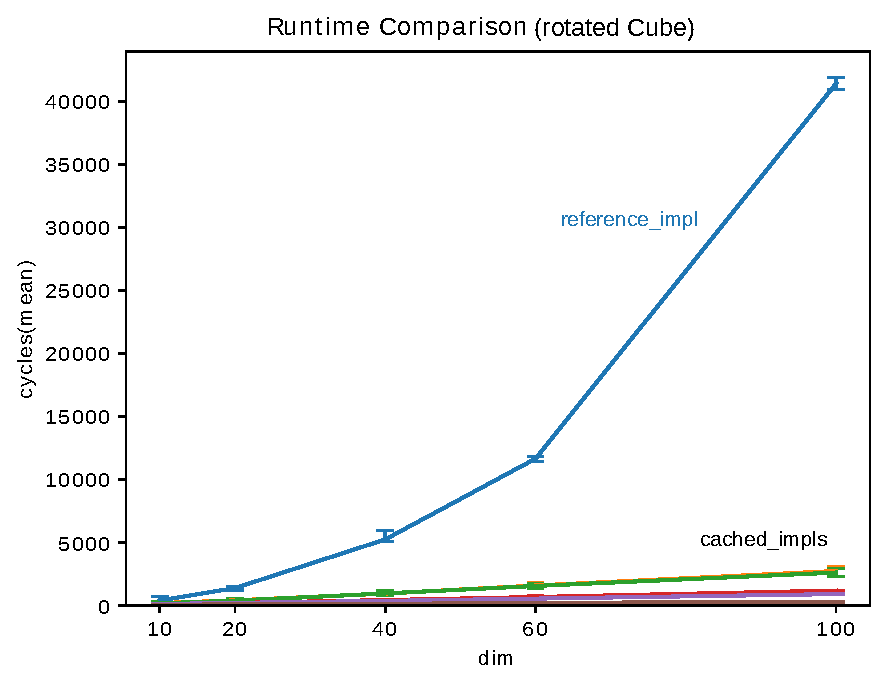
\includegraphics[scale=0.7]{polytopeT_1.eps}
	\end{center}
\end{frame}

\begin{frame}{Benchmark: Intersect}
	\begin{center}
	    \includegraphics[scale=0.7]{polytopeT_2.pdf}
	\end{center}
\end{frame}

\begin{frame}{Benchmark: Intersect}
	\begin{center}
	    \includegraphics[scale=0.7]{polytopeT_3.pdf}
	\end{center}
\end{frame}


\begin{frame}[t]{Sparse Scenario}
	\begin{itemize}
	    \item So far, we considered dense constraint matrices
	    \onslide<2->{
	    \item Now assume each constraint contains only a few variables (still NP-hard)
	    }
	\end{itemize}
	\begin{center}
	    \only<3>{
	    \quad\quad\quad\quad\quad\quad\quad\quad
	    \quad\quad\quad\quad
	    \includegraphics[scale=0.27]{sparsity/motivation0.eps}
	    }
	    \only<4>{
	    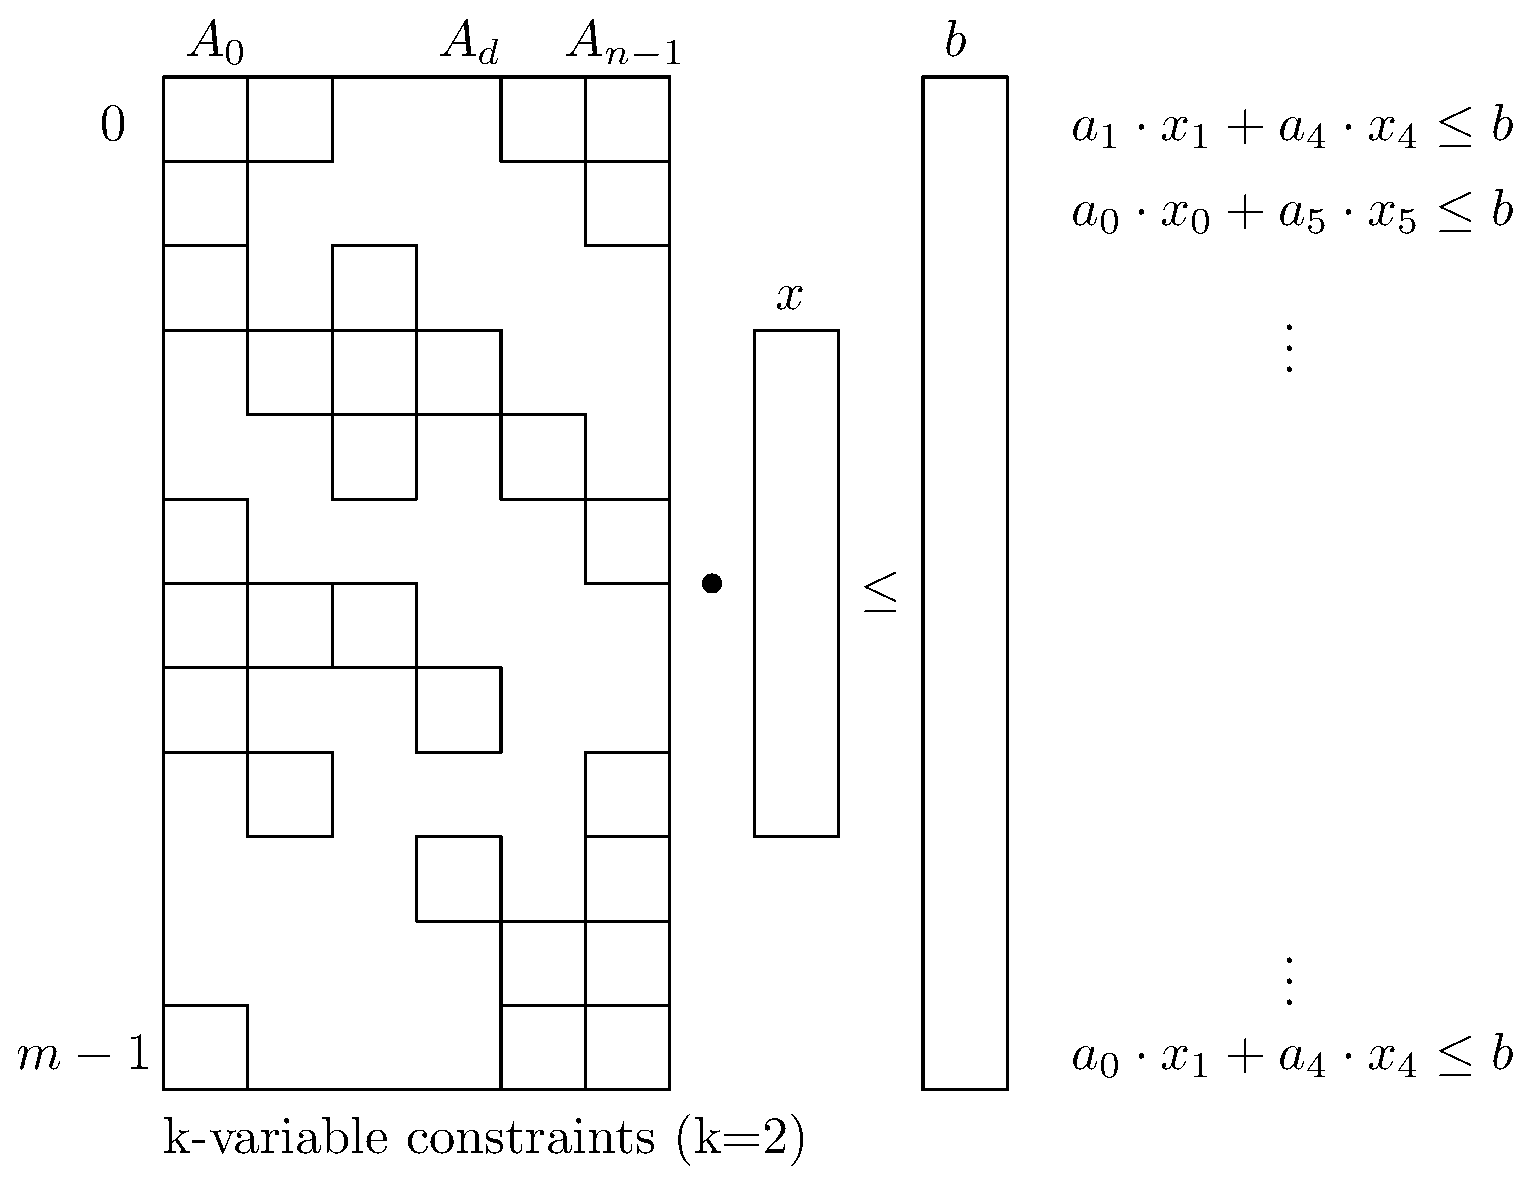
\includegraphics[scale=0.27]{sparsity/motivation1.eps}
	    }
	\end{center}
\end{frame}

\begin{frame}[t]{Sparsity CSC}
	\begin{itemize}
	    \item Sparse matrix format, column major.
	\end{itemize}
	\\[3.4ex]
	\begin{center}
	    \includegraphics[width=90mm]{sparsity/csc.eps}
	\end{center}
\end{frame}

\begin{frame}[t]{Sparsity JIT}
	\begin{itemize}
	    \item Run same matrix many times: kernel?
	    \item Generate code at run time (just-in-time). No blendv, no cmp.
	\end{itemize}
	\begin{center}
	    \includegraphics[width=90mm]{sparsity/jit.eps}
	\end{center}
\end{frame}


\begin{frame}{Benchmark: Runtime Density}
	\begin{center}
	    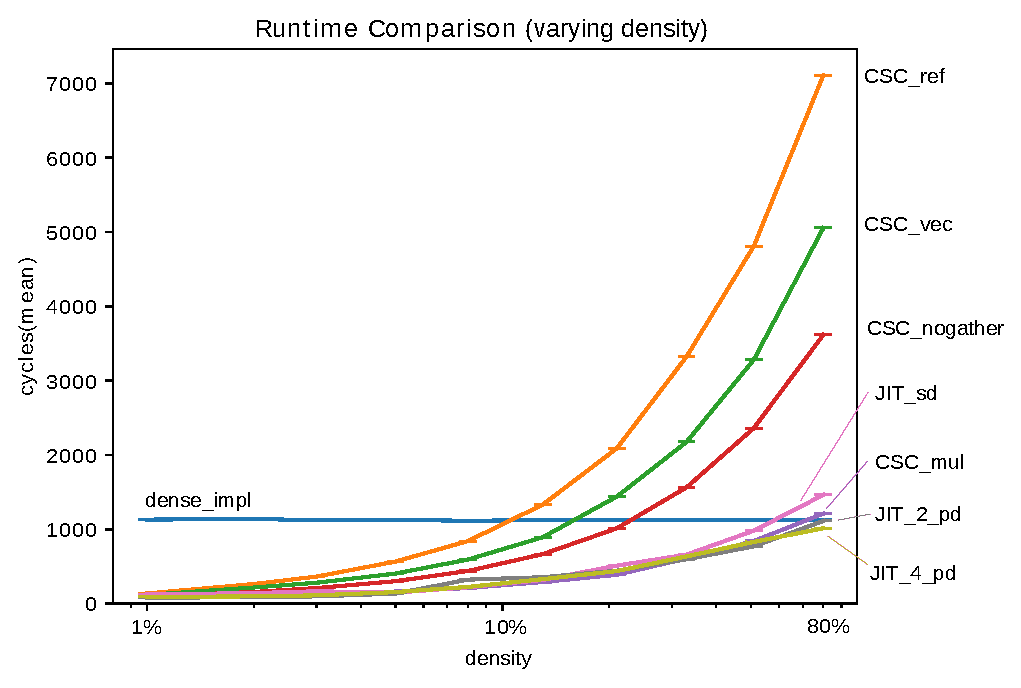
\includegraphics[scale=0.67]{plots/csc_jit_runtime.eps}
	\end{center}
\end{frame}

\begin{frame}{Benchmark: Roofline Density}
	\begin{center}
	    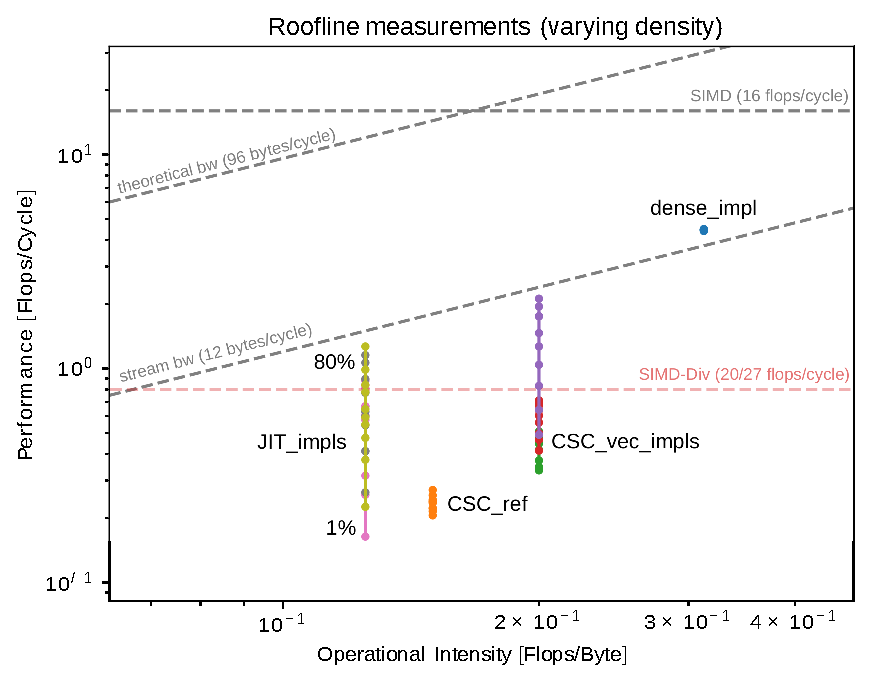
\includegraphics[scale=0.7]{plots/csc_jit_roofline.eps}
	\end{center}
\end{frame}


\begin{frame}{Benchmark: Runtime Latency}
	\begin{center}
	    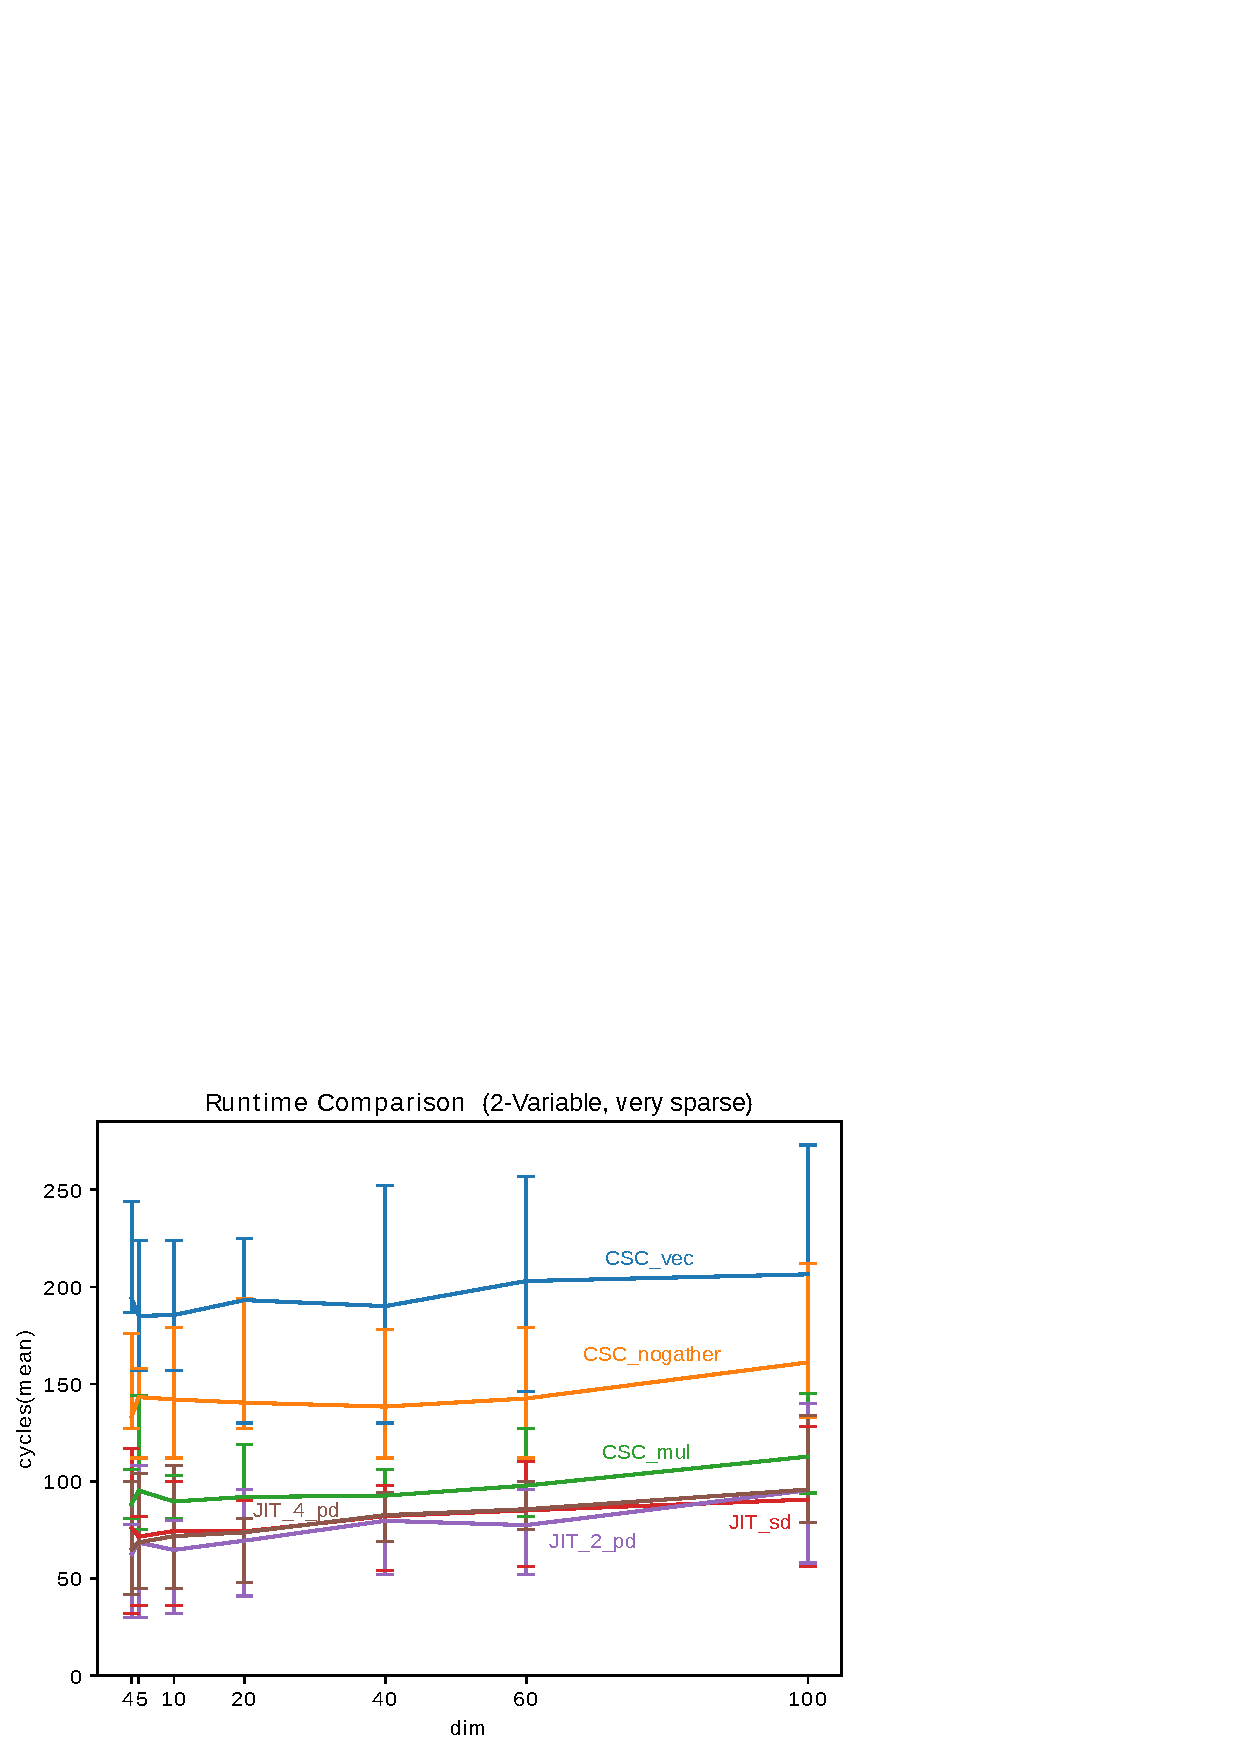
\includegraphics[scale=0.7]{plots/2var_runtime.pdf}
	\end{center}
\end{frame}


\begin{frame}{End}
	\begin{center}
	Thank you very much! \\
	
	\end{center}
\end{frame}



\backupbegin

\begin{frame}{Benchmark: Dense Update}
	\begin{center}
	    \includegraphics[scale=0.7]{polytopeT_4.pdf}
	\end{center}
\end{frame}


\backupend

\end{document}
